% Created by Bonita Graham
% Last update: December 2019 By Kestutis Bendinskas

% Authors: 
% Please do not make changes to the preamble until after the solid line of %s.
\documentclass[12pt]{article}
\usepackage[explicit]{titlesec}
\setlength{\parindent}{0pt}
\setlength{\parskip}{1em}
\usepackage{hyphenat}
\usepackage{ragged2e}
\usepackage{float}
\usepackage[justification=centering]{caption}
\usepackage{listings}
 \usepackage{xcolor} 
 \definecolor{mygreen}{rgb}{0,0.6,0}
 \definecolor{mygray}{rgb}{0.5,0.5,0.5}
 \definecolor{mymauve}{rgb}{0.58,0,0.82}
 \lstset{extendedchars=false} 
 \lstset{ %
 	backgroundcolor=\color{white},      % choose the background color
 	basicstyle=\footnotesize\ttfamily,  % size of fonts used for the code
 	columns=fullflexible,
 	tabsize=4,
 	breaklines=true,               % automatic line breaking only at whitespace
 	captionpos=b,                  % sets the caption-position to bottom
 	commentstyle=\color{mygreen},  % comment style
 	escapeinside={\%*}{*)},        % if you want to add LaTeX within your code
 	keywordstyle=\color{blue},     % keyword style
 	stringstyle=\color{mymauve}\ttfamily,  % string literal style
 	frame=single,
 	rulesepcolor=\color{red!20!green!20!blue!20},
 	% identifierstyle=\color{red},
 	extendedchars=false,
 	language=Python,
 }
\usepackage[colorlinks,linkcolor=blue]{hyperref}
\justifying  

% These commands change the font. If you do not have Garamond on your computer, you will need to install it.
\usepackage{garamondx}
\usepackage[T1]{fontenc}
\usepackage{amsmath, amsthm}
\usepackage{graphicx}

% This adjusts the underline to be in keeping with word processors.
\usepackage{soul}
\setul{.6pt}{.4pt}


% The following sets margins to 1 in. on top and bottom and .75 in on left and right, and remove page numbers.
\usepackage{geometry}
\geometry{vmargin={1in,1in}, hmargin={1.25in, 1.25in}}
\usepackage{fancyhdr}
%\pagestyle{fancy}
%\pagenumbering{gobble}
%\renewcommand{\headrulewidth}{0.0pt}
%\renewcommand{\footrulewidth}{0.0pt}

% These Commands create the label style for tables, figures and equations.
\usepackage[labelfont={footnotesize,bf} , textfont=footnotesize]{caption}
\captionsetup{labelformat=simple, labelsep=period}
\newcommand\num{\addtocounter{equation}{1}\tag{\theequation}}
\renewcommand{\theequation}{\arabic{equation}}
\makeatletter
\renewcommand\tagform@[1]{\maketag@@@ {\ignorespaces {\footnotesize{\textbf{Equation}}} #1.\unskip \@@italiccorr }}
\makeatother
\setlength{\intextsep}{10pt}
\setlength{\abovecaptionskip}{2pt}
\setlength{\belowcaptionskip}{-10pt}

\renewcommand{\textfraction}{0.10}
\renewcommand{\topfraction}{0.85}
\renewcommand{\bottomfraction}{0.85}
\renewcommand{\floatpagefraction}{0.90}

% These commands set the paragraph and line spacing
\titleformat{\section}
  {\normalfont}{\thesection}{1em}{\MakeUppercase{\textbf{#1}}}
\titlespacing\section{0pt}{0pt}{-10pt}
\titleformat{\subsection}
  {\normalfont}{\thesubsection}{1em}{\textit{#1}}
\titlespacing\subsection{0pt}{0pt}{-8pt}
\renewcommand{\baselinestretch}{1.15}

% This designs the title display style for the maketitle command
\makeatletter
\newcommand\sixteen{\@setfontsize\sixteen{17pt}{6}}
\renewcommand{\maketitle}{\bgroup\setlength{\parindent}{0pt}
\begin{flushleft}
\sixteen\bfseries \@title
\medskip
\end{flushleft}
\textit{\@author}
\egroup}
\makeatother

% This styles the bibliography and citations.
%\usepackage[biblabel]{cite}
\usepackage[sort&compress]{natbib}
\setlength\bibindent{2em}
\makeatletter
\renewcommand\@biblabel[1]{\textbf{#1.}\hfill}
\makeatother
\renewcommand{\citenumfont}[1]{\textbf{#1}}
\bibpunct{}{}{,~}{s}{,}{,}
\setlength{\bibsep}{0pt plus 0.3ex}




%%%%%%%%%%%%%%%%%%%%%%%%%%%%%%%%%%%%%%%%%%%%%%%%%

% Authors: Add additional packages and new commands here.  
% Limit your use of new commands and special formatting.

% Place your title below. Use Title Capitalization.
\title{Evaluation of Protein Sub-cellular Localization Using High-throughput Micrographs}

% Add author information below. Communicating author is indicated by an asterisk, the affiliation is shown by superscripted lower case letter if several affiliations need to be noted.
\author{
Wangjie Zheng$^{a}$, Xinyu Jia$^{a}$, Yixiang Qu$^{a}$, Yunzhe Jiang*$^{a}$, Zhizhuo Zhang$^{a}$  \\ \medskip 
$^{a}$ Department of Bioinformatics and Biostatistics, School of Life Sciences and Biotechnology, Shanghai Jiao Tong University, Shanghai, China \\  \medskip 
jiangyunzhe@sjtu.edu.cn* (indicated by asterisk which e-mail for primary communication) 
}
\pagestyle{empty}
\begin{document}
% Makes the title and author information appear.
\vspace*{.12 in}
\maketitle
\vspace{.12 in}
% Abstracts are required.
\section*{abstract}
\par Protein sub-cellular localization plays an important role in systems biology. The visualization technology of gene expression in living cells have emerged dramatically. With the help of deep learning, it becomes possible to handle with astronomical high-throughput micrographs, classifying proteins into different sub-cellular localization. Here, we introduced a deep learning model based on ResNet-18 classifying proteins into twelve categories with the accuracy of 87.66\%. Moving forward, we successfully calculated the size of sub-cells based solely on the red channel. 
% Keywords are required.
\section*{keywords} 
\par Protein Sub-cellular Localization; Green Fluorescent Protein (GFP); Convolutional Neural Network (CNN); Image Processing
\section*{introduction}
\par It is known to all that the regulation of most biological processes are associated with changes in protein abundance and localization. Determination of protein sub-cellular localization facilities understanding post-transnational modifications, protein stability and protein-protein interactions~\cite{chong2015yeast}.
\par Previous large-scale analyses of protein localization in \textit{S. cerevisiae} have depended on transposon-mediated random epitope tagging and plasmid-based over-expression of epitope-tagged proteins~\cite{ross1999large}, which can interrupt important localization signals, leading to abnormal sub-cellular localization. To circumvent these potential problems, green fluorescent protein (GFP) is tagged at the carboxy terminal end by inserting the coding sequence in-frame immediately preceding the stop codon of each ORF~\cite{huh2003global} as Figure~\ref{fig:gfp} displays. It is proved that with this strategy, wild-type levels and patterns of protein expression are minimally perturbed. Furthermore, because GFP fluorescence does not require external cofactors, GFP signal can be monitored in living cells without disrupting cellular integrity. To efficiently quantify the abundance and localization of the about 4,100 visible fusion proteins in the ORF-GFP collection in yeast, cytosolic red fluorescent protein (RFP), a marker of cell boundaries, is introduced into the ORF-GFP array by synthetic genetic array (SGA) technology.
\begin{figure}[!htbp]
\centering
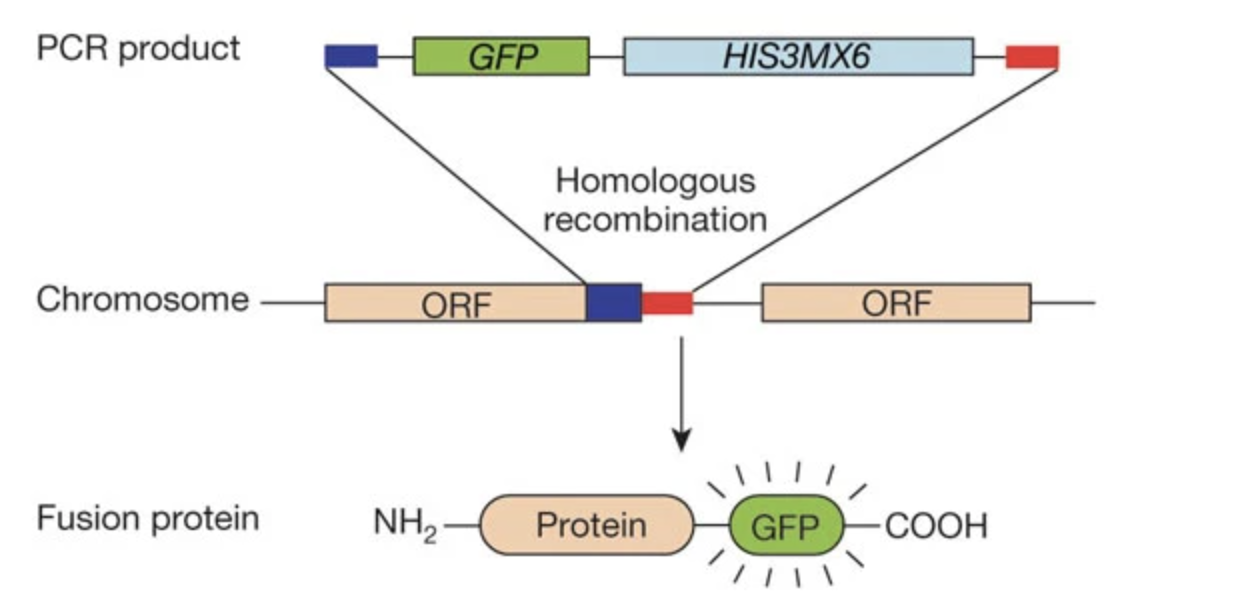
\includegraphics[width=0.6\textwidth]{1.png}
\caption{Strategy of Constructing GFP-tagged proteins}
\label{fig:gfp}
\end{figure}
\par Huh \textit{et al.}~\cite{huh2003global} classified these proteins, representing 75\% of the yeast proteome, into 22 distinct sub-cellular localization categories using wide-field microscopy and manual inspection, and provided localization information for 70\% of previously unlocalized proteins. Benanti \textit{et al.}~\cite{benanti2007proteomic} developed a proteomic screening method that used high-throughput quantitative microscopy of a two-color system to comprehensively screen for ubiquitin-ligase substrates.  Mazumder \textit{et al.}~\cite{mazumder2013single} assayed the transcriptional response of the ribonucleotide reductase (RNR) subunit genes by imaging single transcripts with fluorescence in situ hybridization
(FISH) and subsequently combined this technique with
immunofluorescence detection of Rnr proteins to simultaneously
investigate their translational responses in the same individual
cells as a function of the cell cycle. However, all these methods relied on manual assessment of localization, which is non-quantitative and suboptimal since assignments made by different individuals can be subject to biases and are not powerful enough to deal with astronomical imaging data.
\par With the rapid development of machine learning and conforming booming imaging data, it is imperative to apply automated approaches to analyze protein localization in yeast. Unsupervised algorithm based on clustering was proposed to construct and compare quantitative signatures of protein sub-cellular localization patterns~\cite{loo2014quantitative}. Moving forward, in terms of supervised learning, Chong \textit{et al.}~\cite{chong2015yeast} developed an ensemble of binary classifiers based on support vector machine (SVM) to generate localization data from single-cell measurements and constructed maps of about 3,000 proteins connected to sixteen localization classes on a genome scale.
\par Compared with machine learning, there is no denying that convolutional neural network (CNN) are expert on computer vision and pattern recognition. Much of the success of deep neural networks has been accredited to additional layers because it is these layers that progressively learn more complex features. Deeper neural networks are more difficult to train. ResNet presents a residual learning framework to ease the training of networks that are substantially deeper than those used
previously~\cite{he2016deep}. Typical ResNet models are implemented with double- or triple- layer skips that contain non-linearities (ReLU) and batch normalization in between.
\par Here, we introduced a model based on a pre-trained ResNet-18 to classify protein into twelve sub-cellular localization categories in a systematic and quantitative fashion on a genome scale. It is proved that accuracy of our model increased dramatically compared with those of machine learning models~\cite{chong2015yeast}. Moving forward, we also calculated sizes of different cells in pixel based on the red channel of high-throughput micrographs.

\section*{methods and procedures}
\subsection*{Image classification}
The labeled datasets we used in this project contain 65000 images for training, 12500 images for testing and 12500 images for validation. In order to reach a satisfied accuracy towards images to be classified, we choose to use Convolutional Neural Network as classifier. Before fully optimizing the model, we construct two simple models with limited number of convolutional layers, as shown in Figure \ref{simplenet}.
\begin{figure}[ht!]
\centering
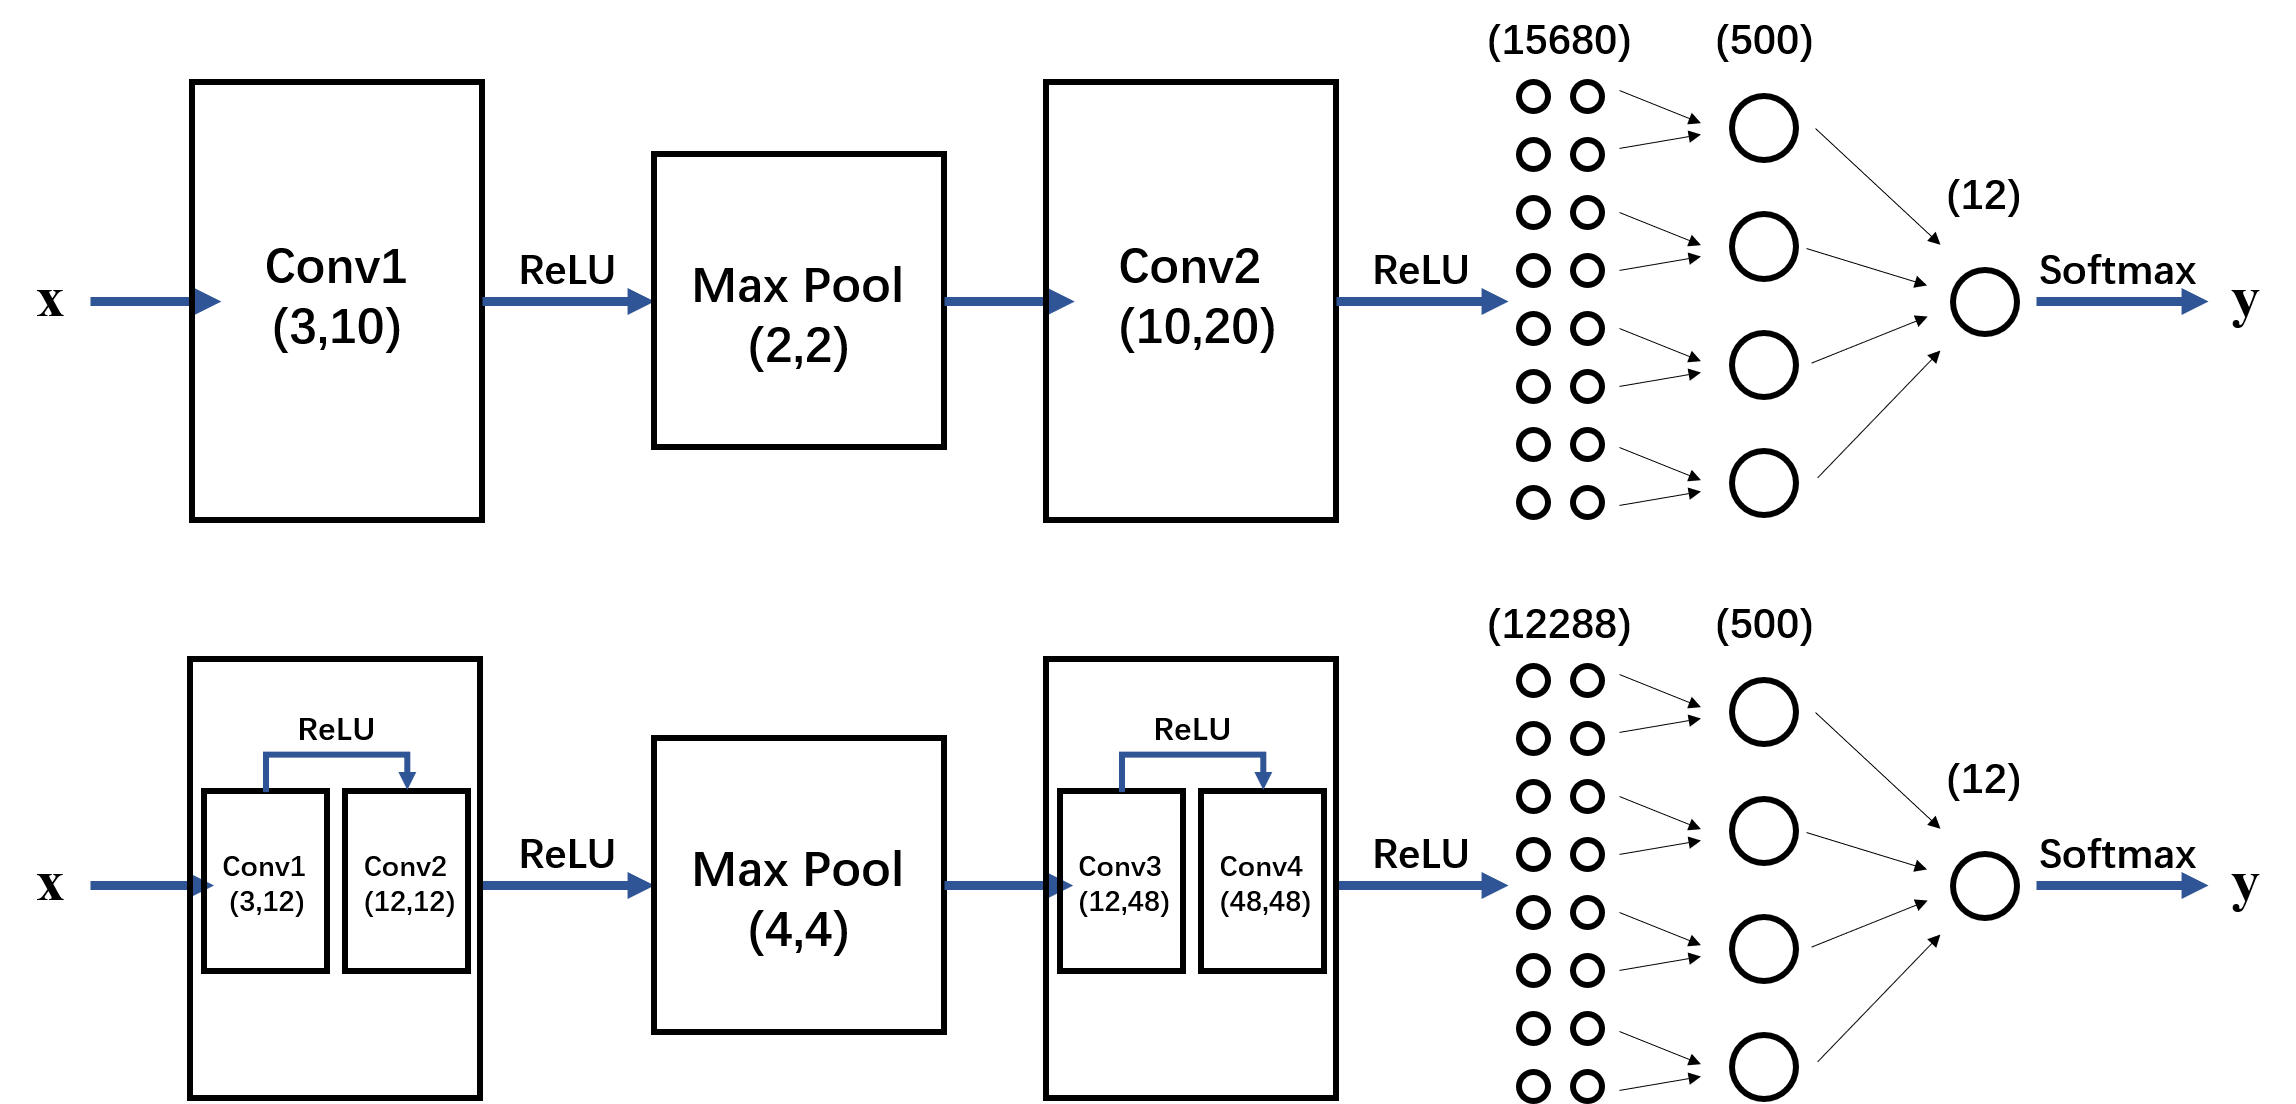
\includegraphics[width=0.8\textwidth]{simplenet.png}
\caption{Two \textit{SimpleNet} CNN nerworks we use at the beginning}
\label{simplenet}
\end{figure}
\par
However, optimizing models with simple structures couldn't achieve our goal of a higher accuracy. Therefore, we moved on to the idea of optimizing a complex network.
\par
In 2012, Krizhevsky \textit{et al}\cite{krizhevsky2012imagenet}. rolled out the red carpet for the Deep Convolutional Neural Network. This was the first time this architecture was more successful that traditional, hand-crafted feature learning on the ImageNet. Their DCNN, named AlexNet, contained 8 neural network layers, 5 convolutional and 3 fully-connected. This laid the foundational for the traditional CNN, a convolutional layer followed by an activation function followed by a max pooling operation. Much of the success of Deep Neural Networks has been accredited to these additional layers. The intuition behind their function is that these layers progressively learn more complex features. And our Simplenet models are also based on this idea.Despite the popular meme shared in AI communities from the Inception movie stating that "We need to go Deeper", He \textit{et al}\cite{he2016deep}. empirically show that there is a maximum threshold for depth with the traditional CNN model, shown as Figure \ref{threshold}.
\begin{figure}[ht!]
\centering
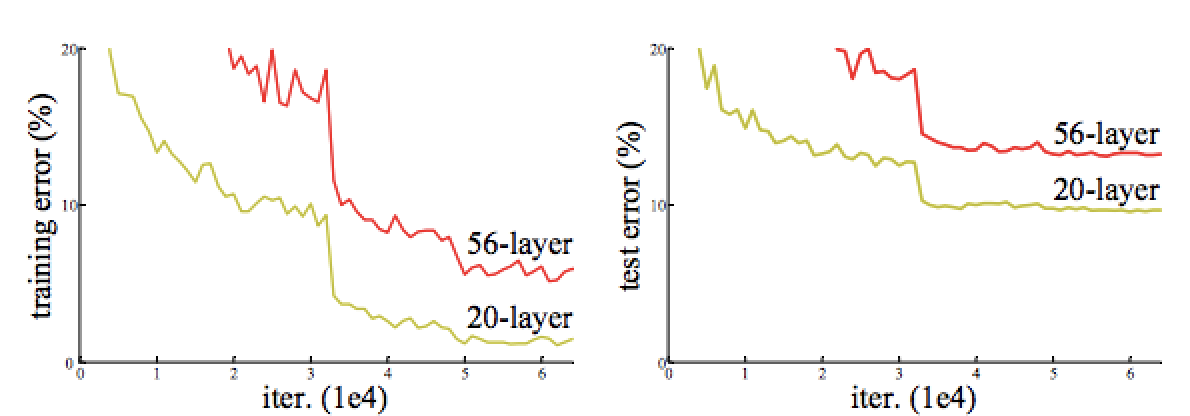
\includegraphics[width=0.7\textwidth]{threshold.png}
\caption{The deeper network has higher training error, and thus test error}
\label{threshold}
\end{figure}
\par The failure of the 56-layer CNN could be blamed on the optimization function, initialization of the network, or the famous vanishing/exploding gradient problem. Amongst the many theories explaining why Deeper Networks fail to perform better than their Shallow counterparts, it is sometimes better to look for empirical results for explanation and work backwards from there. The problem of training very deep networks has been alleviated with the introduction of a new neural network layer - \textbf{The Residual Block}\cite{he2016deep}.
\begin{figure}[H]
\centering
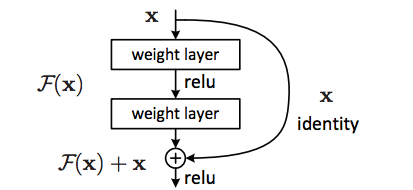
\includegraphics[width=0.6\textwidth]{resnet.png}
\caption{Residual learning: a building block}
\label{resnet}
\end{figure}
\par Figure \ref{resnet} shows the most important thing to learn from this article. For developers looking to quickly implement this and test it out, the most important modification to understand is the \textit{Skip Connection}, identity mapping. This identity mapping does not have any parameters and is just there to add the output from the previous layer to the layer ahead. However, sometimes x and F(x) will not have the same dimension. The identity mapping is multiplied by a linear projection W to expand the channels of shortcut to match the residual. This allows for the input x and F(x) to be combined as input to the next layer, which is shown as follows,
$$
\mathbf{y}=\mathcal{F}\left(\mathbf{x},\left\{W_{i}\right\}\right)+W_{s} \mathbf{x}
$$
\par The Skip Connections between layers add the outputs from previous layers to the outputs of stacked layers. This results in the ability to train much deeper networks than what was previously possible. Therefore, we decided to construct a ResNet neural network based on the high-performance ResNet. As Figure \ref{model} shows, there are several ResNet structures that are widely used. We choose to use simple but effective 18-layer ResNet to build the skeleton of our model.
\begin{figure}[h]
\centering
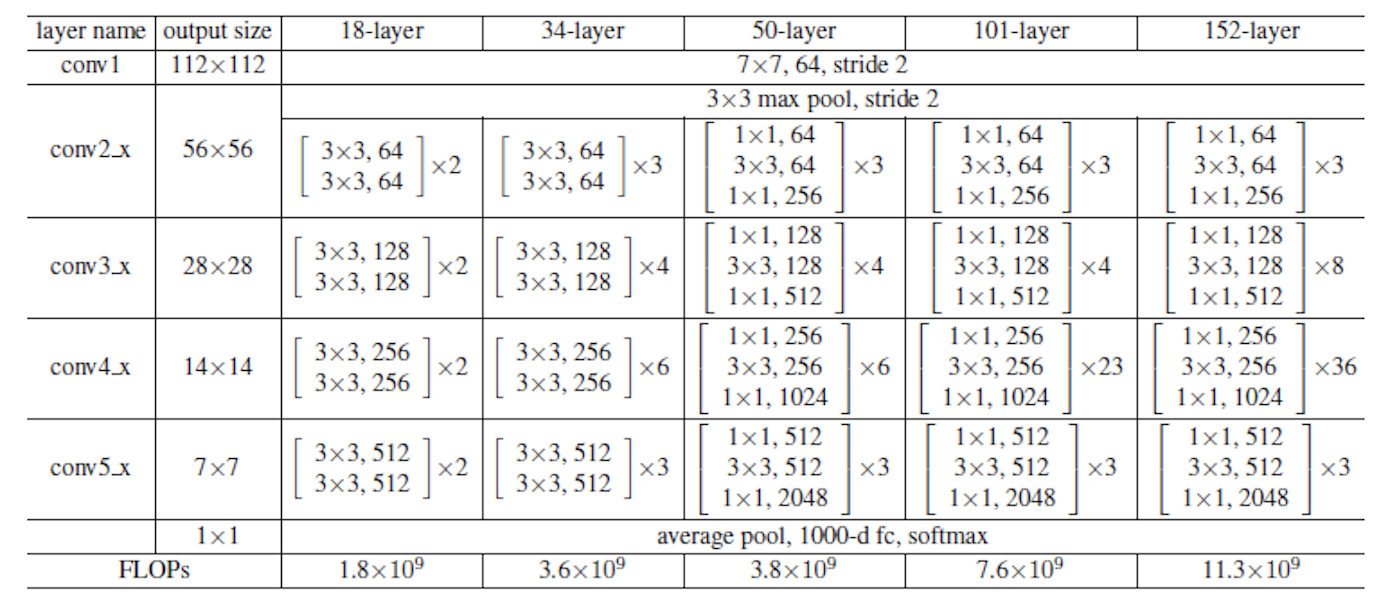
\includegraphics[width=0.9\textwidth]{model.png}
\caption{Different ResNet models}
\label{model}
\end{figure}
\par In order to make the model better fit our data and increase the accuracy for the test data, we modified the 18-layer ResNet and added two convolutional layers before conventional ResNet-18, which proved to have great performance in our dataset, not only the 3-channel input, but also 2-channel and 1-channel input.
\par Considering that all of these images in our dataset are with B channels equaling to zero, 3-channel (RGB) input is the same as 2-channel input. But to make our result more convincing, we applied the same model on RG channels input and G channel input.
\subsection*{Calculation of sub-cell size}
\par Since RFP is a marker of cell boundaries, we wanted to explore whether the size of the cell could be estimated solely based on the area covered by RFP. We compared sizes of sub-cells (in pixel) in red channel with the real sizes (in pixel) to determine whether it is feasible that the RFP marked boundaries of cells.In terms of determining the boundary contour of the sub-cells in the image, we chose to use OpenCV package in Python, including functions \lstinline|cv2.threshold()|, \lstinline|cv2.findContours()| and \lstinline|cv2.drawContours()|.
\par The function of \lstinline|cv2.threshold()| is to binarize the image. If pixel value is greater than a threshold value, it is assigned one value (may be white), else it is assigned another value (may be black).  Binarization of image is to set the gray value of the pixels on the image to 0 or 255, which makes the whole image show a clear black and white effect. In digital image processing, the binary image plays an important role. Binarization of image can significantly reduces the amount of data in the image, thereby highlighting the outline of the target. If an image has a uniform gray value, and is on a uniform background with other levels of gray value, the binarization can reach a comparative segmentation effect. If the difference between the image and the background is not in the gray value, difference features can be converted into a gray difference, and then use the threshold selection to segment the image. By dynamically adjusting the threshold to realize the binarization of the image, the specific result of the segmented image can be dynamically observed.
\par The function of \lstinline|cv2.findContours()| is to automatically identify the contours of objects aligned with chromatic aberration and mark them by setting parameters and thresholds. The figure is not necessarily the exact figure used to recognize the outline, and in fact, it can be any figure. In the study, we got the outline of images of the red channel, and finally drew the outline on the original images so that it can be a more effective fashion.
\par There is another problem in identifying contours of images. The resolution of the boundaries in all images were heterogeneous so that there could not be a constant threshold. To handle with problem, we found that the resolution of the outline could be increased by adjusting contrast. \lstinline|ImageEnhance.Contrast()| can adjust image contrast. An enhancement factor of 0.0 gives a solid grey image, and a factor of 1.0 gives the original image. Gamma correction is a nonlinear operation used to encode and decode luminance or tristimulus values in image identification. Gamma correction is defined by the following power-law expression,
$$
V_{\text {out }}=A V_{\text {in }}^{\gamma}
$$
It was suggested that the relative resolution of the outline was increased to a certain extent by increasing the contrast of the picture. When the outline was identified, size of sub-cells can be calculated by \lstinline|contourArea| function in OpenCV package.
\section*{results}
\subsection*{Image classification}
\par At the beginning of our work, we introduced two \textit{SimpleNet} models. After a training process with 30 epoches, the two models gave out less satisfied accuracy results, 71.7\% and 75.8\% respectively. These results prompted us to turn to complex networks - ResNet.After several adjustments on model's parameters, the image classification result for ResNet was really promising, which reached the accuracy of nearly 90\%. 
\par In order to compare the difference between 2-channel input and 1-channel input, we trained the same model with different number of channels input. The results of training for each epoch are shown in Figure \ref{training_results}.
\begin{figure}[H]
\centering
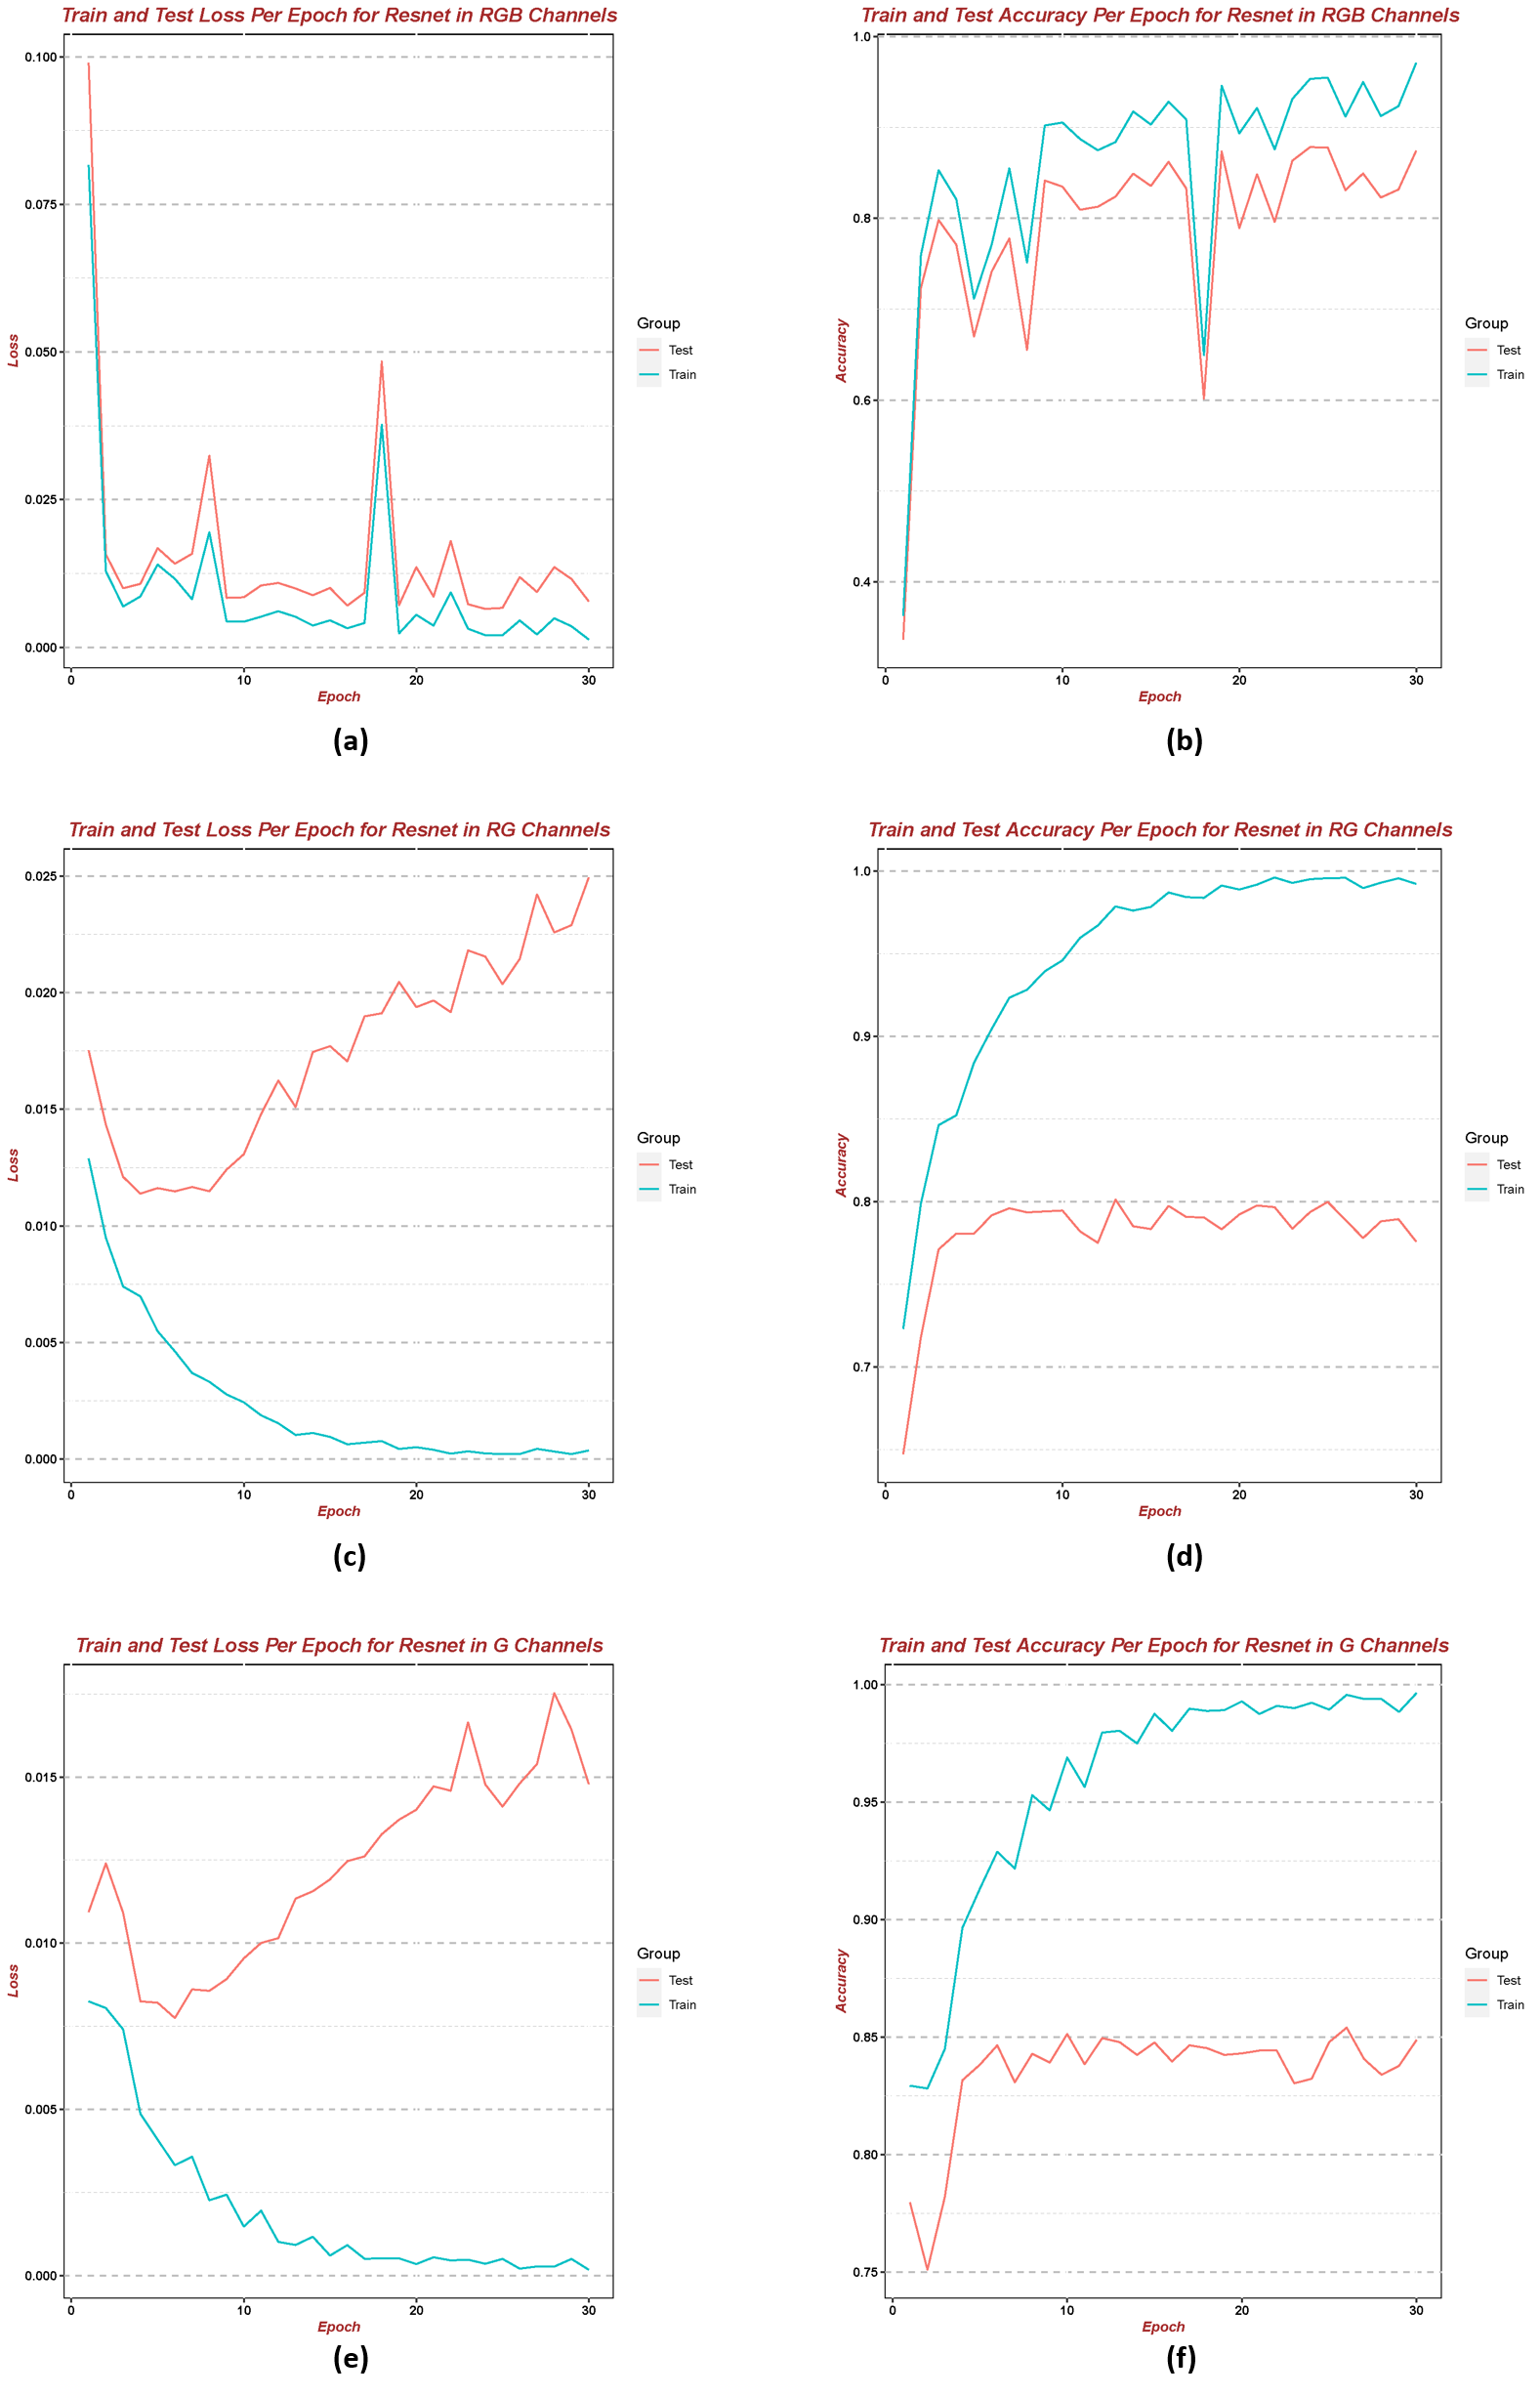
\includegraphics[width=0.8\textwidth]{training_results.png}
\caption{The result comparison between different input channels. \protect\\
(a) and (b) are Loss and Accuracy of RGB input.\protect\\
(c) and (d) are Loss and Accuracy of RG input.\protect\\
(e) and (f) are Loss and Accuracy of G input.\protect\\}
\label{training_results}
\end{figure}
\par It seems clear that when providing the original RGB channels, both training and testing losses were decreasing and their accuracy increased with the same trend. The rather small difference between training and testing losses indicated the very good fit of the model. But, as for the other two situations, while the training loss decreased and accuracy increased continually, their testing losses kept increasing and their accuracy stayed unchanged after a small number of epoches. This abnormality indicated the early overfit of the model, which brought up a possibility that a large amount of information was ignored with the loss of several channels.
\par After training, we used validation dataset to evaluate the reliability of our model, the accuracy is shown in Table \ref{accuracy_table}.
\begin{table}[!htbp]
\renewcommand{\arraystretch}{1.2}
\centering
\caption{The validation results of three different input channels}
\begin{tabular}{|c|c|c|c|}
\hline
{\color[HTML]{000000} \textbf{Input channels}} & {\color[HTML]{000000} RGB}     & {\color[HTML]{000000} RG}      & {\color[HTML]{000000} G}       \\\hline
{\color[HTML]{000000} \textbf{Accuracy}}       & {\color[HTML]{000000} 87.66\%} & {\color[HTML]{000000} 78.82\%} & {\color[HTML]{000000} 82.74\%}\\ \hline
\end{tabular}
\label{accuracy_table}
\end{table}
\subsection*{Calculation of sub-cell size}
\par From the images randomly selected from the training set, whatever class of sub-cell is, 
the cell contour image after extracting the red channel was generally the same as that of the original image. Figure~\ref{fig:comp} displays the comparison of two kinds of images. The first row displays raw images and the second raw displays images extracted the red channel. Therefore, we believed that it was feasible to estimate the size of the cells through the area covered by the RFP.
\begin{figure}[!htbp]
    \centering
    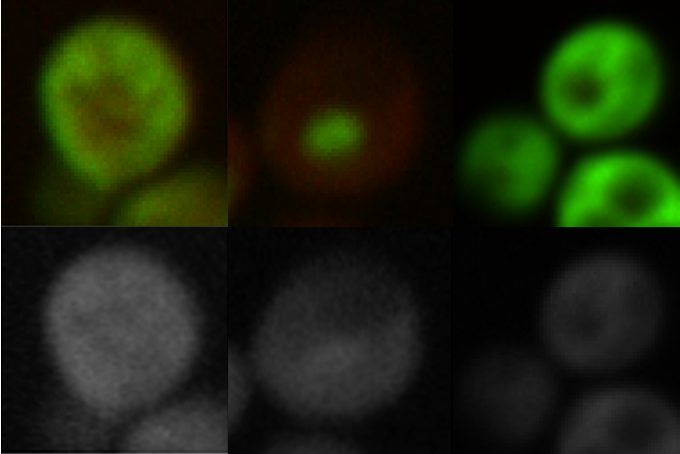
\includegraphics[width=0.6\textwidth]{3.png}
    \caption{Comparison between images extracted red channel and the original images}
    \label{fig:comp}
\end{figure}
\par In order to identify outline of sub-cell, a threshold should be set as a parameter of functions. When the threshold was set to 127 as default, the so-called outline picture was merely clear. We thought that it was because that red boundary was not obvious enough. We gradually reduced the threshold from 50 to 20, hoping to find a optimal value. Figure~\ref{fig:outline} displays the contour identified by the function at different threshold.
\begin{figure}[!htbp]
    \centering
    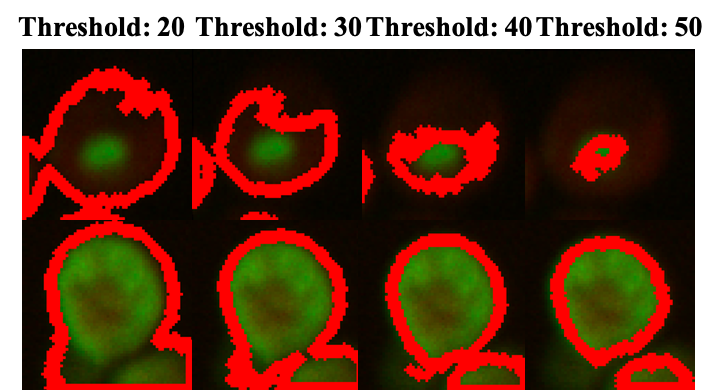
\includegraphics[width=0.7\textwidth]{4.png}
    \caption{Different threshold set to identify the outline of sub-cells}
    \label{fig:outline}
\end{figure}
\par It was interesting that though in a small range of threshold (from 20 to 50), the outline of the first image changed dramatically (the first row). However, the outline of the second image seemed insensitive to the change of threshold. As for the first image, the smaller the threshold was, the more accurate the image was outlined.  As for the second image, the larger the threshold was, the more accurate the area was outlined. It was suggested that the blurriness of the outline of different images was distinct, so that the boundary threshold could not be a constant. We concluded that if only the red channel was used for contour drawing, the threshold must vary from images.
\par We sought adjusting contrast of images to clearly identify outlines. In order to determine at what level contrast of images should be reset, Figure~\ref{fig:contrast} displays the relationship between the area and the threshold at a specific contrast value.
\begin{figure}[!htbp]
    \centering
    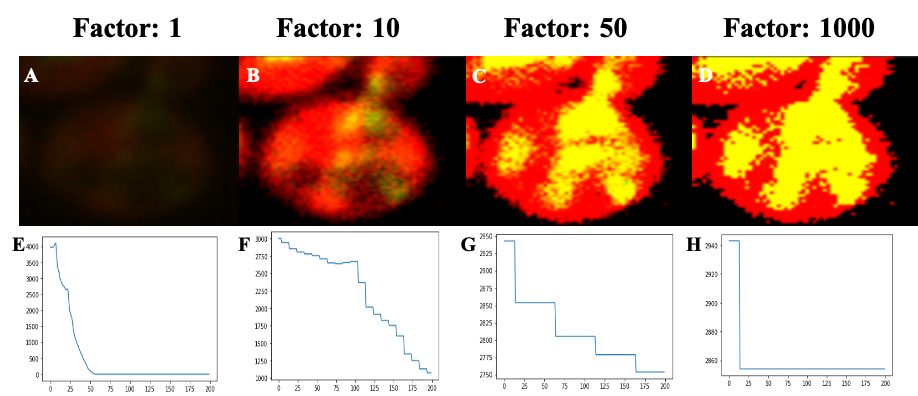
\includegraphics[width=0.95\textwidth]{5.png}
    \caption{Relationship between the area and the threshold at a specific factor of contrast value (above)}
    \label{fig:contrast}
\end{figure}
\par It was noticeable that after enhancing the contrast, the area could be calculated under different thresholds (\textbf{E} and \textbf{F} in Figure~\ref{fig:contrast}). However, we were unable to determine the exact threshold yet. Ideally, the area should be independent of the threshold. We argued that the reason of inconsistent change of the curve in Figure~\ref{fig:contrast}-\textbf{F} lay in the model detected the a sharp change between the targeted and the background. The higher the contrast value we set, the larger difference in color contrast was likely to be. Compared with Figure~\ref{fig:contrast}-\textbf{F}, \ref{fig:contrast}-\textbf{G} and Figure~\ref{fig:contrast}-\textbf{H}, it is clear that the more the contrast is enhanced, the less the area change under different thresholds. 
\par For each test image, we calculated the area of covered by the red channel based on the enhanced contrast (1000 times). The outline boundary of the sub-cell was conspicuous, and the area converged at some thresholds.
\section*{discussion}
\par Comparing to the previous research~\cite{chong2015yeast} that our datasets come from, our model shows a tremendous progress on the accuracy of classifying the images with a nearly 20\% improvement. It shows the powerful ability of Convolutional Neural Network in image classification.
\par The reason why we choose ResNet-18 as the skeleton of our model was mainly its effectiveness. However, its simplicity can also implicates the limitation of performance. The performance of the model might be higher if we try other ResNet models such as ResNet-50 or even, if we have enough time and computing resources, ResNet-152.
\par Considering the blue channel is of no use in the model, the RGB-input model could be seen as an example of binary-channel model. Therefore, the experiment showed that the test accuracy of the single-channel is smaller than that of binary-channel. The reason for this is about the design of the datasets, we suggest, that the red channel gives the information of cell boundary and the G channel gives the information of product mark. If we use only G channel to train our model, the loss of the information about the relative position between cell and product will influence the outcome of the model. But with the price of lower accuracy, the advantage of single-channel input is a much faster training step. In short, while giving up some information, a faster training process is as compensation.
\par Though by enhancing the contrast of images, we were able to identify outline easily, there were some exceptions. As Figure~\ref{fig:excep-1} displays, there is no clear sub-cell boundary. When we tried to get outline by enhancing contrast, the model is likely to use the slight color difference of the background to extract an outline boundary deliberately so that the enhanced image (right above) was totally messed up. As Figure~\ref{fig:excep-2} displays, there is slight signal of the red channel, which was proved by the enhanced image (right above), so that the calculation based on the red channel was not accurate.
\begin{figure}[!htbp]
\centering
\begin{minipage}[t]{0.48\textwidth}
\centering
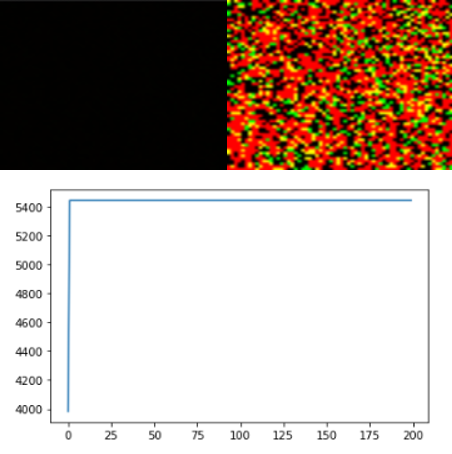
\includegraphics[width=\textwidth]{excep-1.png}
\caption{No sub-cell boundary}
\label{fig:excep-1}
\end{minipage}
\begin{minipage}[t]{0.48\textwidth}
\centering
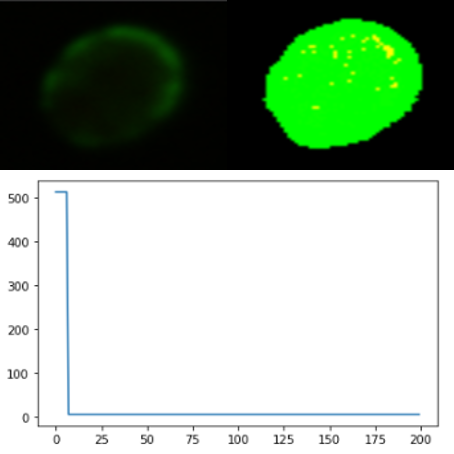
\includegraphics[width=\textwidth]{excep-2.png}
\caption{No signal in red channel}
\label{fig:excep-2}
\end{minipage}
\end{figure}
\par To sum up, the primary reason for the above two exception is that the algorithm cannot detect signal of the red channel. Thus, we cannot calculate the size of sub-cells of which RFP is not expressed. We devised our model to make it more robust so that it can determine whether the size of the input image can be calculated or not. Noticeably, if sizes of sub-cells cannot be calculated based on the red channel, we can calculate them based on the green channel with the same method.
\section*{conclusions}
\begin{enumerate}
\item From our results, we can conclude that ResNet-18 can be used to develop high-performance determination and classification of protein sub-cellular localization.
\item It is clear that ResNet-18 masters not only ternary-channel images but also single-channel and binary-channel images, and our modified ResNet model perform very well in single-channel and binary-channel images, though there are slight problems of over-fitting for the single-channel images.
\item Training speed could be faster by giving up some information (such as channels), but lower accuracy and possible early overfit may be the price. 
\item With the aid of contrast enhancement and image processing algorithms, we are able to identify the contour of sub-cells, and thus calculate the size of sub-cell based on the red channel (RFP).
\end{enumerate}
\newpage
\section*{DATA AND CODE AVAILABILITY}
Please see our \href{https://github.com/quyixiang/BioBigData}{\textbf{GitHub}} for the results, data and code.
\section*{acknowledgements}
\par This work was supported by the Center for HPC at Shanghai Jiao Tong University. We thanked Distinguish Professor Hui Lv and Assistant Researcher Xiaolei Wang from School of Life Sciences and Biotechnology, Shanghai Jiao Tong University for their useful instructions and comments which have greatly improved the manuscript. We were also grateful to T.A. Yan Kong, who accompanied us this semester and replied our questions on the lectures as soon as possible. 
\bibliographystyle{unsrt}
\bibliography{ref}
\end{document}
